\documentclass[french]{beamer}

\usepackage[utf8]{inputenc}
\usepackage[T1]{fontenc}
\usepackage{verbatim}
\usepackage{url}
\usepackage{booktabs}       % professional-quality tables
\usepackage{amsfonts}       % blackboard math symbols
\usepackage{nicefrac}       % compact symbols for 1/2, etc.
%\usepackage{microtype}      % microtypography
\usepackage{amsmath}
\usepackage{caption}
\usepackage[ruled,vlined]{algorithm2e}
\usepackage{graphicx}

\usetheme{Warsaw}


\begin{document}


		\begin{frame}
		\begin{center}
		\Large{\textbf{Breaking News Bandit}}
		\vspace{20pt}
		\end{center}

	\begin{center}
	Achille Aknin \& Alban Pierre

	20th January 2017
	\end{center}
		\end{frame}

	\begin{frame}
		\frametitle{Introduction}
		\textbf{Regular MAB}
		\begin{itemize}
			\item $A$ arms to be pulled at any time $t$
			\item Reward from pulling the arm $a$ follows a law $r \sim L_a$
		\end{itemize}
		\textbf{Breaking News Bandit}
		\begin{itemize}
			\item One arm might give a higher reward than usual at any time: $r \sim L_a(t)$
			with $\mu_a(t)$ possibly very high.
		\end{itemize}
	\end{frame}

	\begin{frame}

		\tableofcontents[]
	\end{frame}


	\begin{frame}
	\frametitle{Data generation}
	\section{Data generation}
	Several states per arms, with a Gaussian distribution
	\begin{itemize}
		\item At most one hot arm for a time $t$
		\item Several hot arms at the same time $t$ possible
	\end{itemize}

	\begin{figure}[h]
			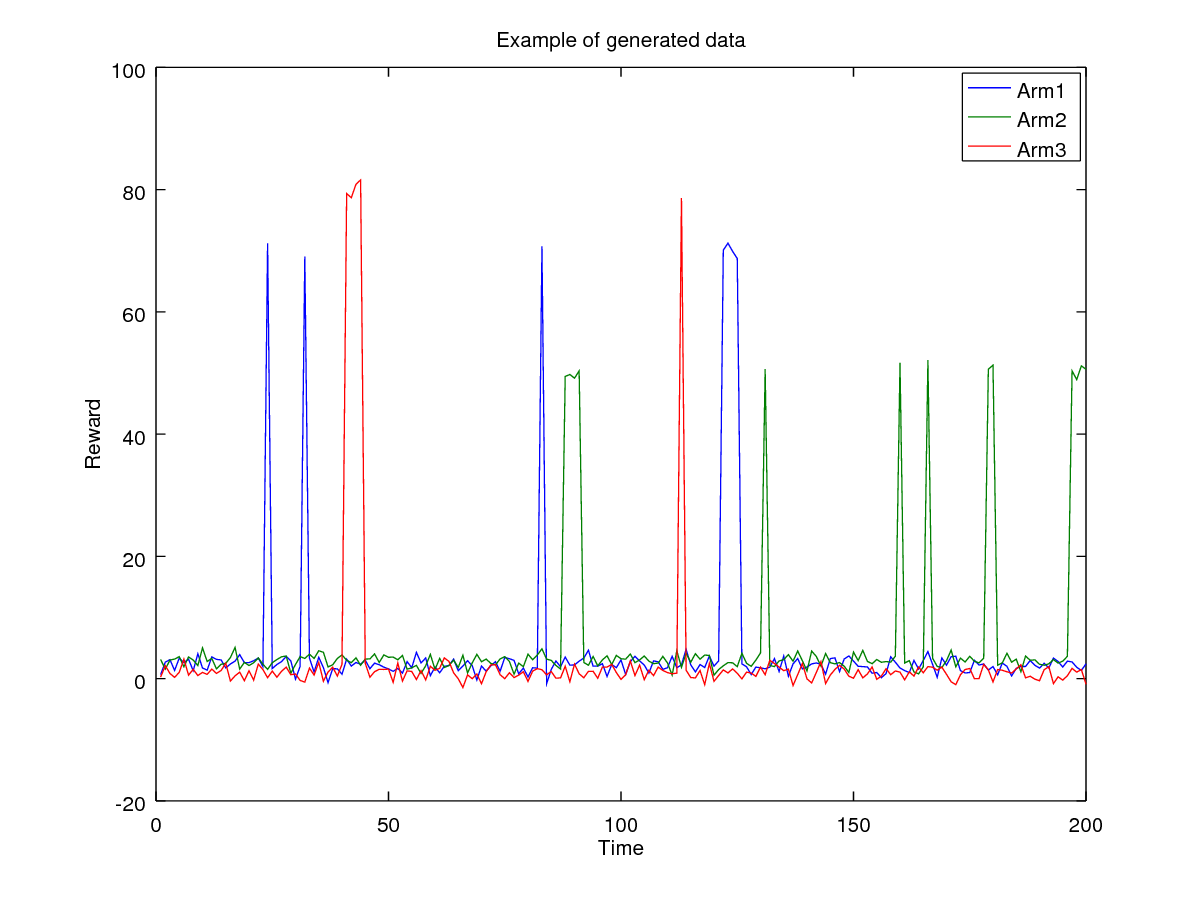
\includegraphics[width=0.7\linewidth]{generated_data_one.png}
			%\caption{Example of generated data}

		\label{fig:f}
	\end{figure}


\end{frame}

\begin{frame}
	\frametitle{Upper Confidence Bound Algorithm}

	\begin{itemize}
		\item Regular MABs: each arm always have the same reward function
		\item At each point choose arm:
		\begin{equation*}
		a^* = argmax_{a} \Big(\hat\mu_a(t) + \sqrt{\frac{log(t)}{2N_a(t)}}\Big)
		\end{equation*}
		\item $\sqrt{\frac{1}{2N_a(t)}}$: confidence on the mean
		\item $log(t)$: promotes trying every arm from time to time
	\end{itemize}


%	\begin{algorithm}
%		\caption{UCB Algorithm}
%		\For{$i=1:T_{max}$}{
%			Compute $a^* = argmax_{a} \Big(\hat\mu_a(t) + \sqrt{\frac{log(t)}{2N_a(t)}}\Big)$\;
%			Draw arm $a^*$ and receive reward $r(t)$\;
%			Update $\hat\mu_{a^*}(t+1) = \frac{N_{a^*}(t)\times \hat\mu_{a^*}(t) + r(t)}{N_{a^*}(t)+1}$\;
%			Update $N_{a^*} = N_{a^*}+1$\;
%		}
%	\end{algorithm}
\end{frame}

\begin{frame}
	\frametitle{Exact probabilities inference with Gaussian Mixture}
	\section{Breaking News MAB Algorithms}
	\subsection{Exact probabilities inference with Gaussian Mixture}

	Tries to be mathematically exact.
	\begin{itemize}
		\item Gaussian mixture (EM algorithm)
		\item Computes probabilities of each state from an observed reward
		\item Computes transition probabilities (gradient descent)
	\newline
	\end{itemize}

	$\rightarrow$ Very long to compute

	$\rightarrow$ Parameters very sensible to little changes

	$\rightarrow$ Takes too much time to get stable parameters

\end{frame}

\begin{frame}
	\frametitle{Intuitions for Breaking News Bandit algorithms}
	\begin{figure}[h]
		\begin{center}
			%\framebox[4.0in]{$\;$}
			%\fbox{\rule[-.5cm]{0cm}{4cm} \rule[-.5cm]{4cm}{0cm}}
			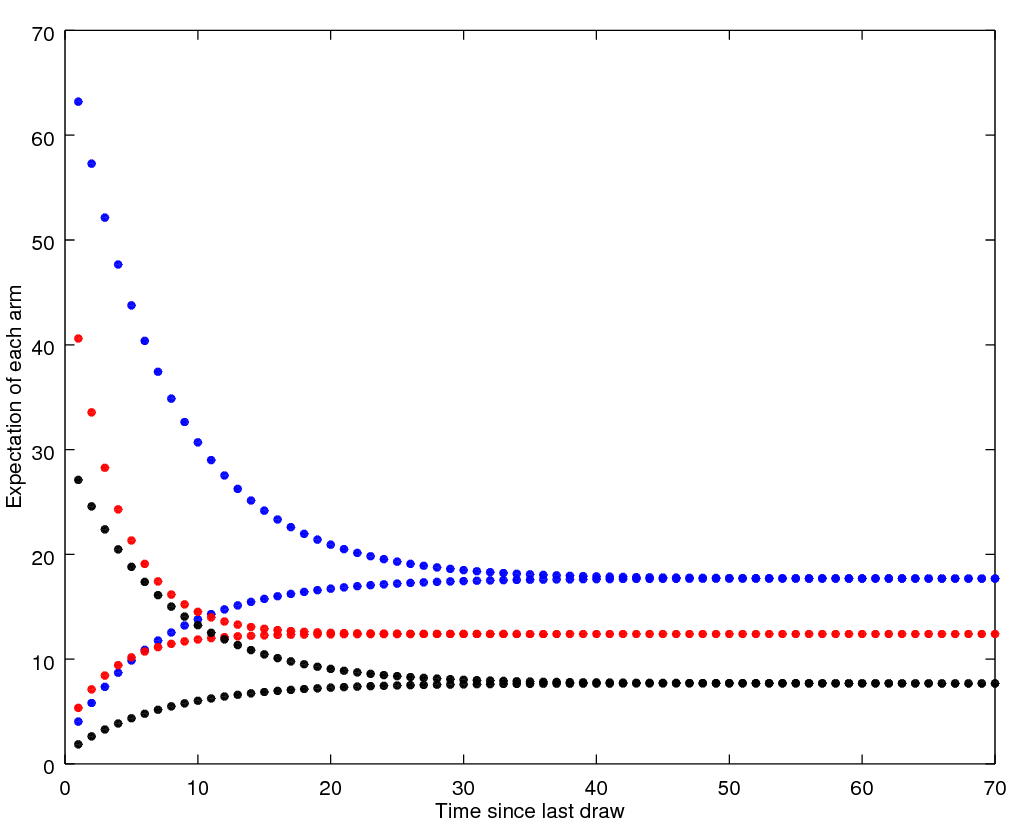
\includegraphics[width=0.78\textwidth]{expectations.png}
		\end{center}
		\caption{Expectation of each arm as a function of time since the last draw}
	\end{figure}

\end{frame}

\begin{frame}
	\frametitle{Nearest Neighbors Upper Confidence Bound Algorithms}

	\subsection{Nearest Neighbors Upper Confidence Bound Algorithms}

	\begin{itemize}
		\item Monte-Carlo estimation
		\item Embeds all previous rewards in a space (Last reward of the arm; Time since last draw) with some convenient deformations.
		\item For a new point, it computes the average expectation of neighbors
	\end{itemize}

\end{frame}

\begin{frame}
	\frametitle{K-Nearest Neighbors Long Term Expectation}

	\subsection{K-Nearest Neighbors Long Term Expectation}

	Tries to have a long term strategy instead of a greedy choose of next draw.
	\newline

	It pulls arms according to the $n$ future rewards (with a decay rate)

\end{frame}

\subsection{UCB\_Var}
\begin{frame}
	\frametitle{UCB\_Var}

	\begin{itemize}
		\item Estimate the maximal value that an arm reward might reach with mean $\hat\mu_a(t)$ and variance $\hat\sigma_a(t)$.
		\item Uncertainty of $\sqrt{\frac{1}{2N_a(t)}}$
		\item Estimation of the range of the rewards from each arm:
		\begin{equation*}
			r \in \Big[\hat\mu_a(t)-\hat\sigma_a(t)-\sqrt{\frac{1}{2N_a(t)}}, \hat\mu_a(t)+\hat\sigma_a(t)+\sqrt{\frac{1}{2N_a(t)}}\Big]
		\end{equation*}
		\item Problem: Quadratic complexity because we need to compute the variance from scratch at each step
	\end{itemize}

\end{frame}

\subsection{UCB\_Max}
\begin{frame}
	\frametitle{UCB\_Max}
	\begin{itemize}
		\item Purpose: Avoid the quadratic complexity
		\item Remember maximal value of each arm $M_a(t)$ instead of variance $\hat\sigma_a(t)$
		\item Faster than UCB\_Var for almost equivalent results
	\end{itemize}
\end{frame}

\begin{frame}
	\frametitle{Time of computation}

	\section{Time of computation and results}

	 At most one hot state, 3 arms * 2 states :
	 \newline


	 	\begin{tabular}{rccccc}
	 		Arms : & TS & UCB & GM & UCB\_KNN & KNN\_LONG \\
	 		Time (sec) : & 7.12 & 2.19 & 1000.5 & 25.39 & 35.85
	 	\end{tabular}
	 	\newline
	 	\newline

	 	\begin{tabular}{rcc}
	 		Arms : & UCB\_MAX & UCB\_VAR \\
	 		Time (sec) : & 3.06 & 5.37
	 	\end{tabular}

\end{frame}

\begin{frame}
	\frametitle{Results (One hot arm, 3 arms * 2 states)}

	\begin{figure}[h]
		\begin{center}
			%\framebox[4.0in]{$\;$}
			%\fbox{\rule[-.5cm]{0cm}{4cm} \rule[-.5cm]{4cm}{0cm}}
			\vspace{-10pt}
			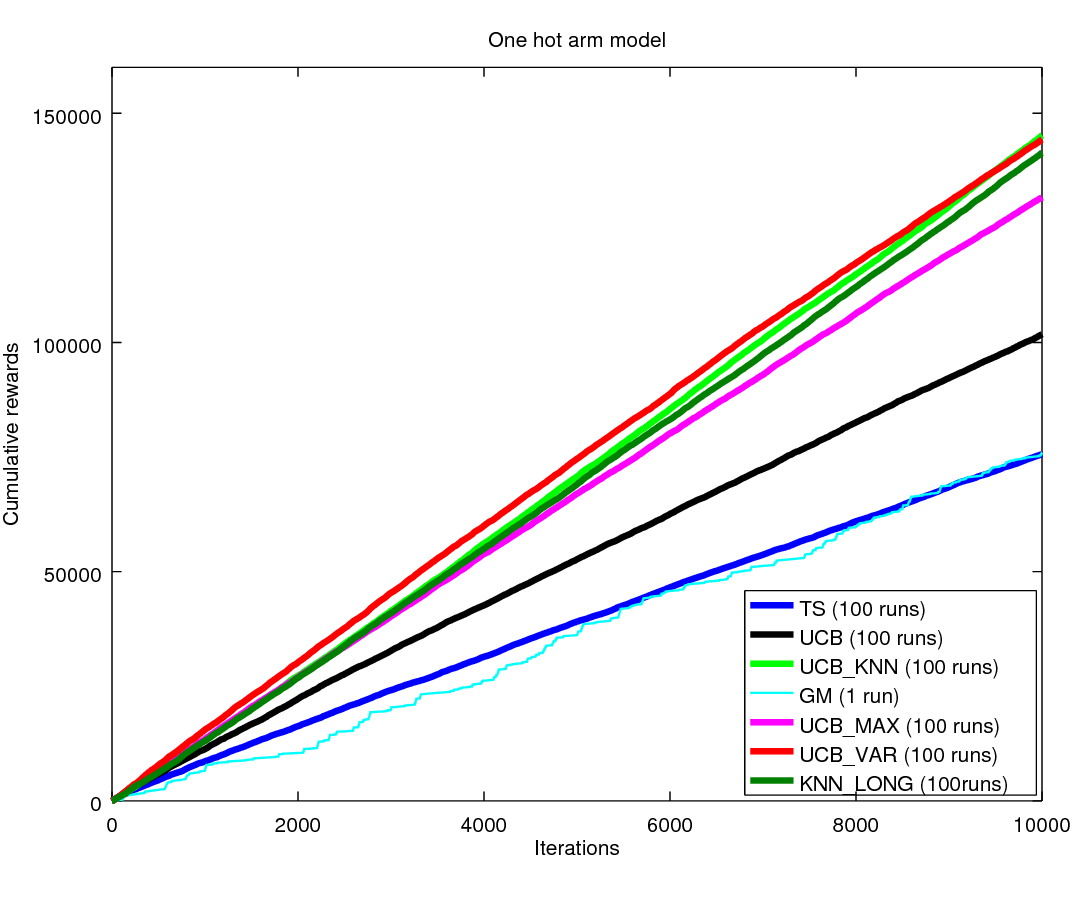
\includegraphics[width=1.05\textheight]{all_10000it.png}

			\vspace{-10pt}
			\centering{\scriptsize{All algorithms for 10000 iterations (3 arms * 2 states, One hot arm)}}
		\end{center}
	\end{figure}
\end{frame}

\begin{frame}
	\frametitle{Results (One hot arm, 3 arms * 2 states)}
	\begin{figure}[h]
		\begin{minipage}[b]{.49\linewidth}
			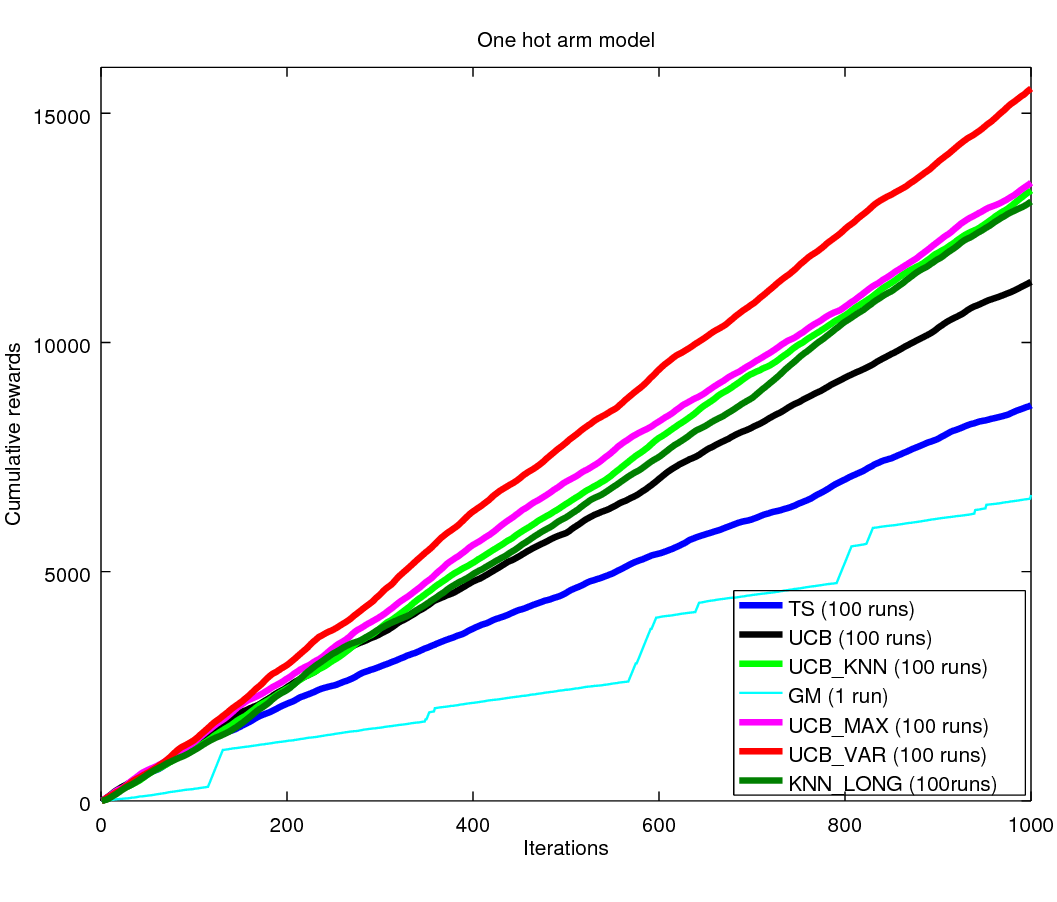
\includegraphics[width=1.0\textwidth]{begin_1000it.png}

			\centering{\scriptsize{1000 first iterations (3*2, one)}}
		\end{minipage}
		\hfill
		\begin{minipage}[b]{0.49\linewidth}
			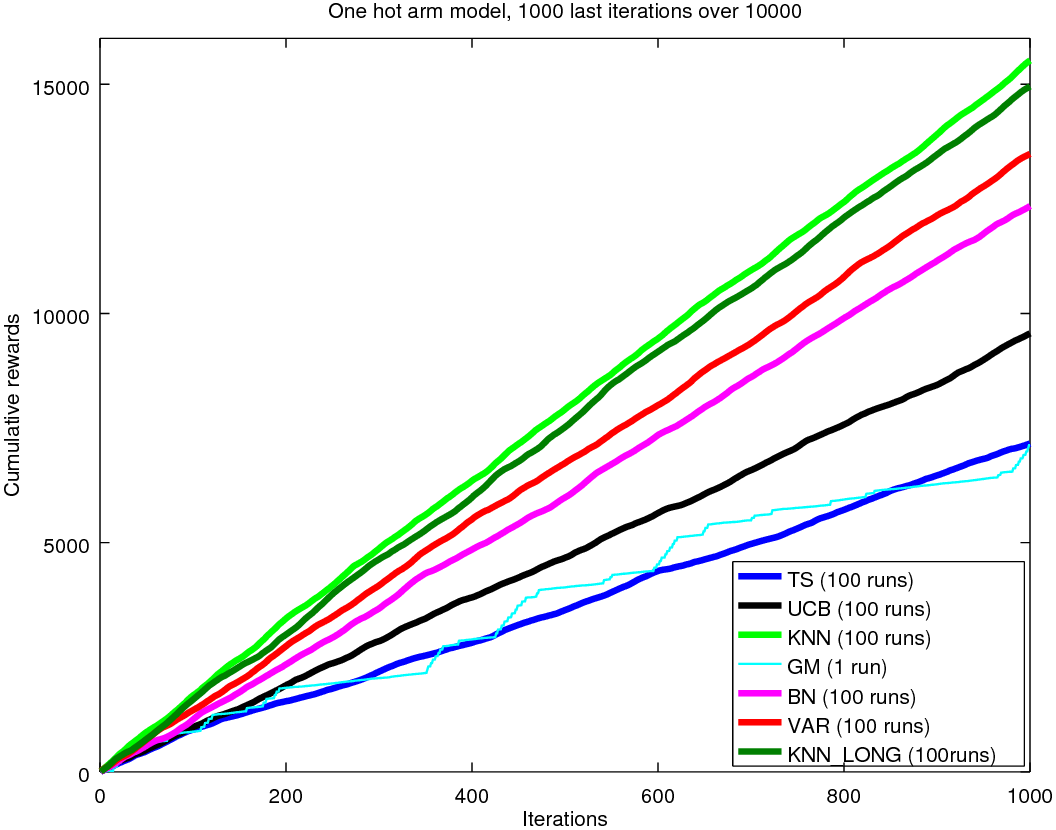
\includegraphics[width=1.0\textwidth]{last_1000it.png}

			\centering{\scriptsize{1000 last iterations (3*2, one)}}
		\end{minipage}
		\label{fig:f}
	\end{figure}

\end{frame}

\begin{frame}
	\frametitle{Results (Several hot arms, 3 arms * 2 states)}

	\begin{figure}[h]
		\begin{center}
			%\framebox[4.0in]{$\;$}
			%\fbox{\rule[-.5cm]{0cm}{4cm} \rule[-.5cm]{4cm}{0cm}}
			\vspace{-10pt}
			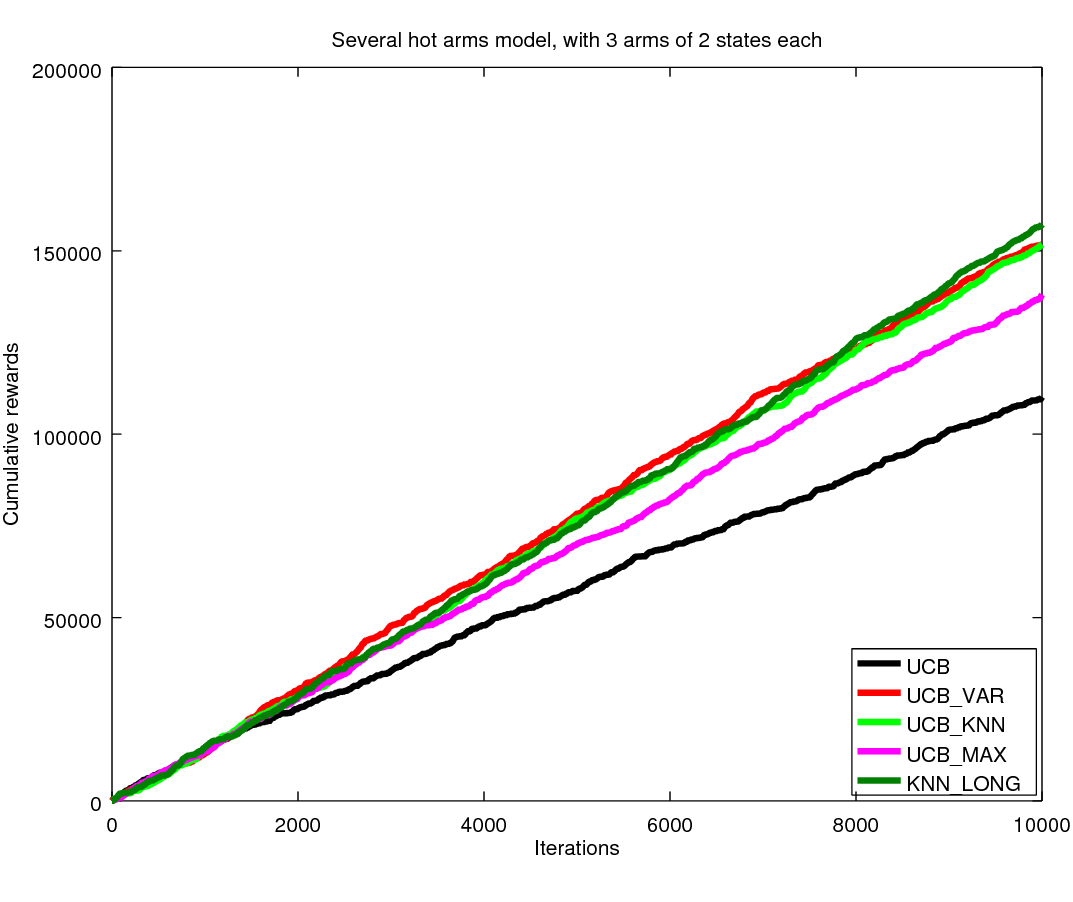
\includegraphics[width=1.05\textheight]{all_m_10000it.png}

			\vspace{-10pt}
			\centering{\scriptsize{All algorithms for 10000 iterations (3 arms * 2 states, several hot arms)}}
		\end{center}
	\end{figure}
\end{frame}

\begin{frame}
	\frametitle{Results (Several hot arms, 3 arms * 2 states)}

	\begin{figure}[h]
		\begin{minipage}[b]{.49\linewidth}
			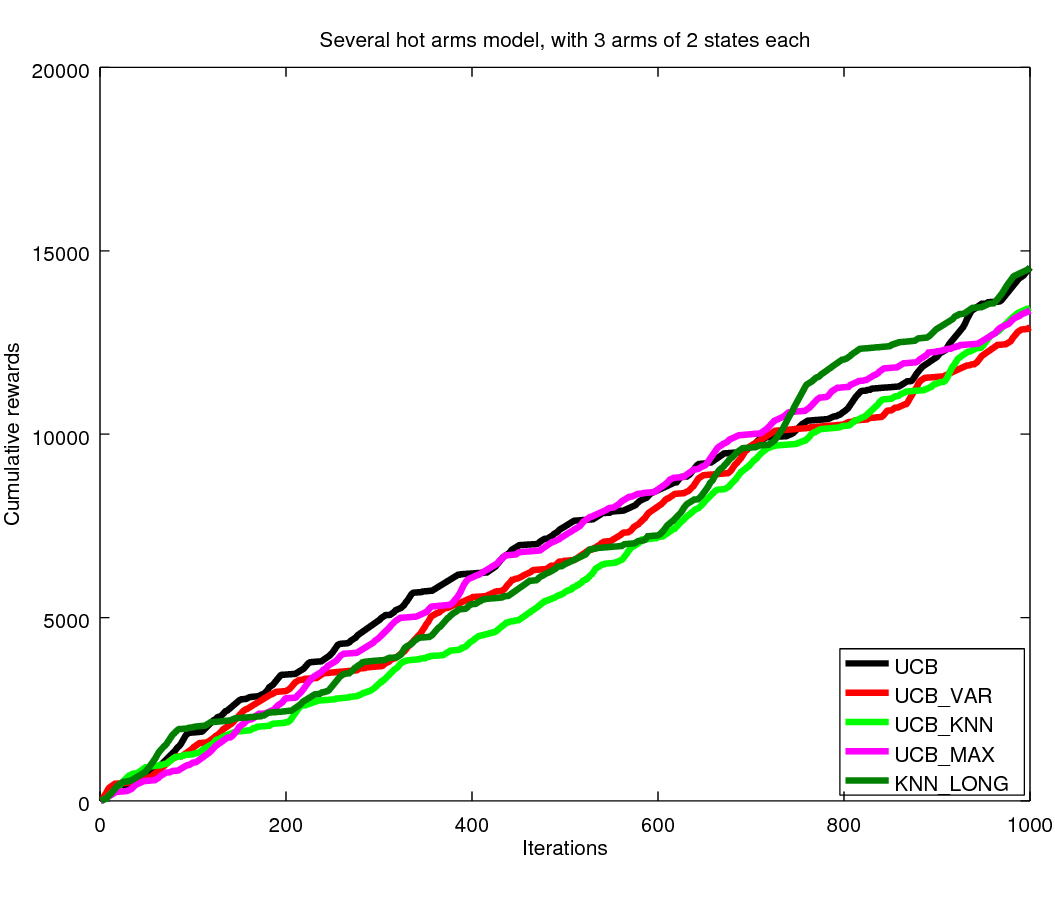
\includegraphics[width=1.0\textwidth]{begin_m_1000it.png}

			\centering{\scriptsize{1000 first iterations (3*2, several)}}
		\end{minipage}
		\hfill
		\begin{minipage}[b]{0.49\linewidth}
			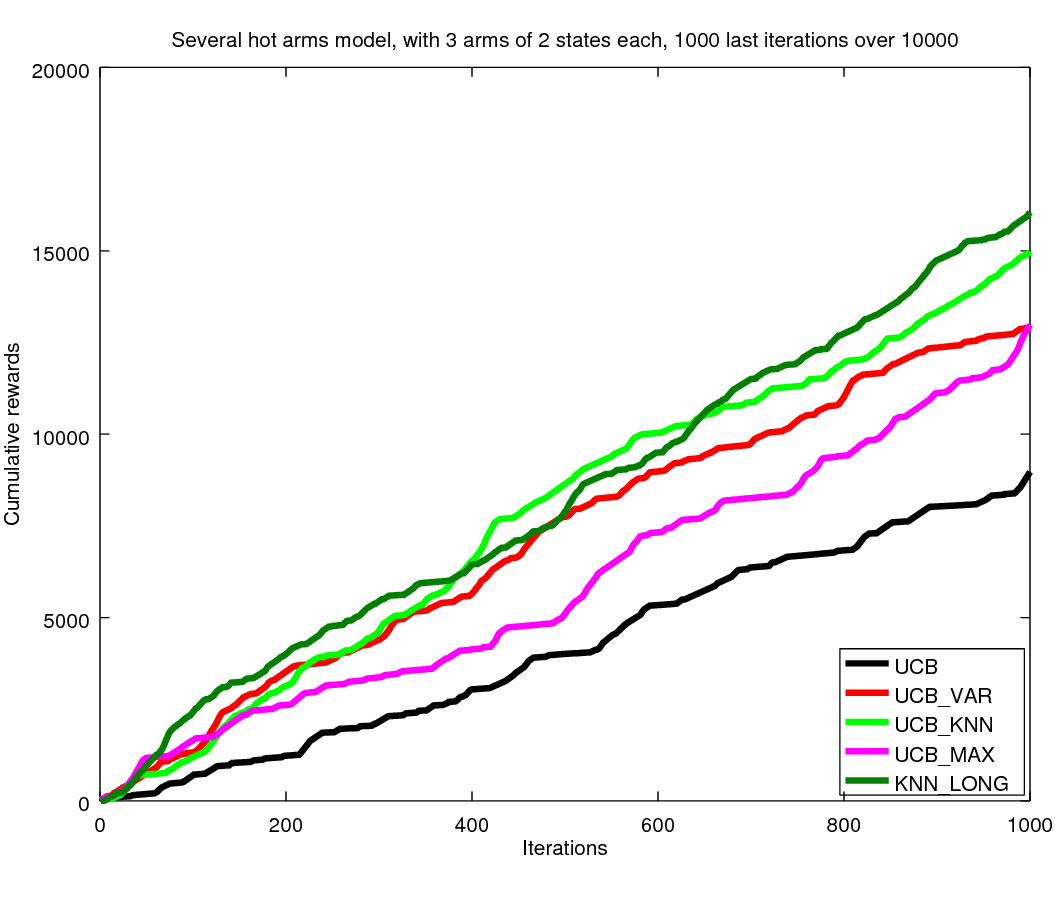
\includegraphics[width=1.0\textwidth]{last_m_1000it.png}

			\centering{\scriptsize{1000 last iterations (3*2, several)}}
		\end{minipage}
		\label{fig:f}
	\end{figure}
\end{frame}

\begin{frame}
	\frametitle{Results (One hot arm, 5 arms * 3 states)}

	\begin{figure}[h]
		\begin{center}
			%\framebox[4.0in]{$\;$}
			%\fbox{\rule[-.5cm]{0cm}{4cm} \rule[-.5cm]{4cm}{0cm}}
			\vspace{-10pt}
			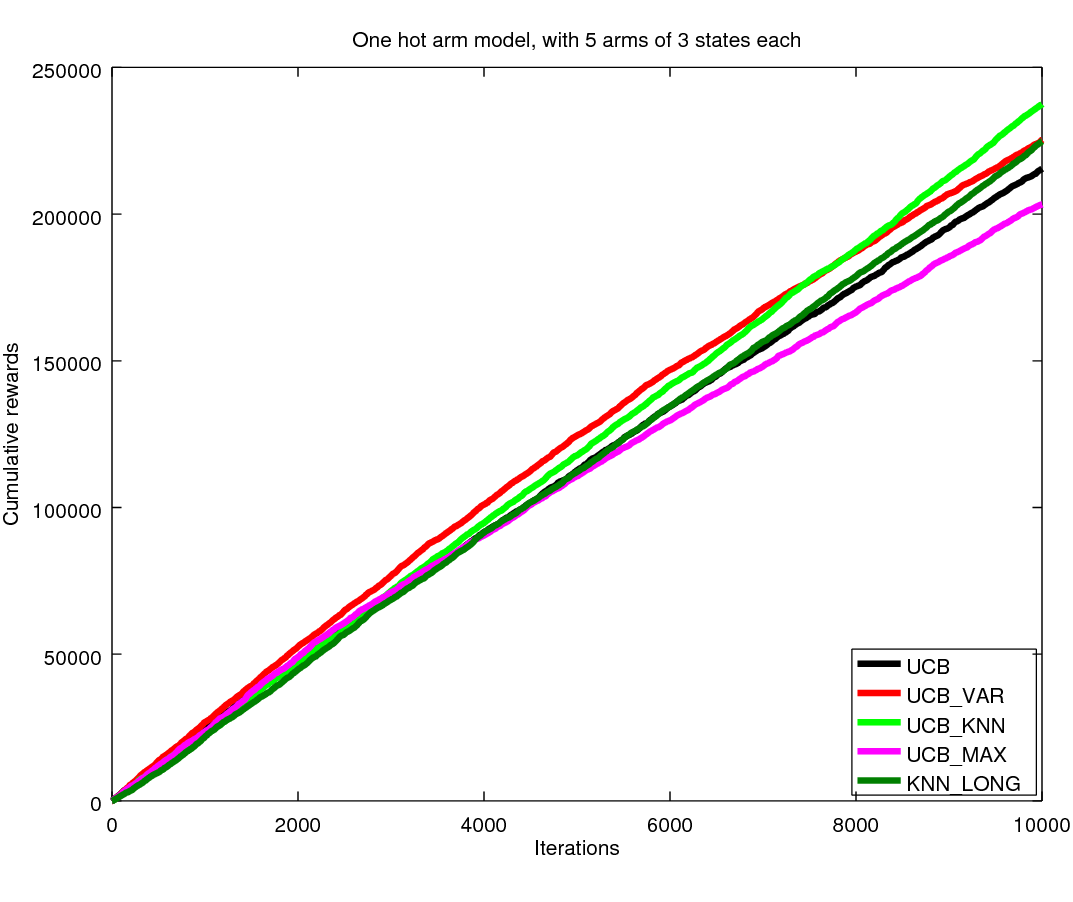
\includegraphics[width=1.05\textheight]{all_s_10000it.png}

			\vspace{-10pt}
			\centering{\scriptsize{All algorithms for 10000 iterations (5 arms * 3 states, at most one hot arm)}}
		\end{center}
	\end{figure}
\end{frame}

\begin{frame}
	\frametitle{Results (One hot arm, 5 arms * 3 states)}

	\begin{figure}[h]
		\begin{minipage}[b]{.49\linewidth}
			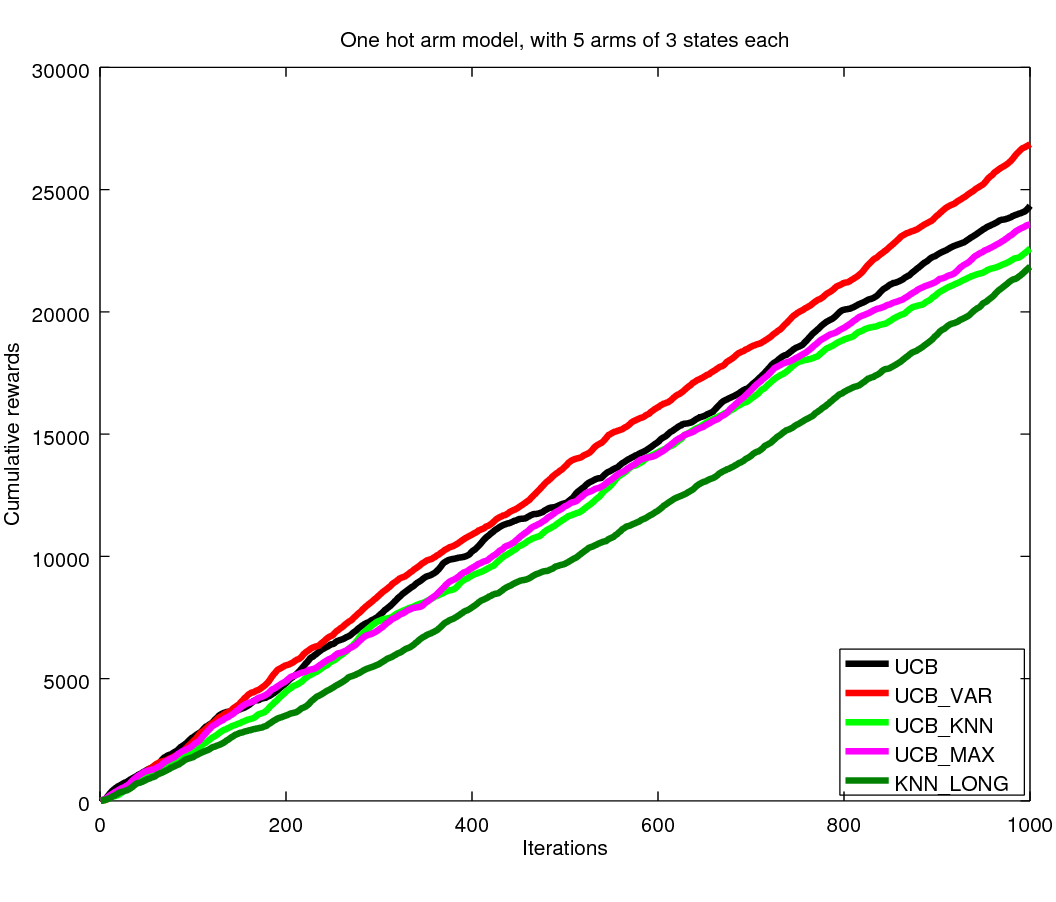
\includegraphics[width=1.0\textwidth]{begin_s_1000it.png}

			\centering{\scriptsize{1000 first iterations (5*3, one)}}
		\end{minipage}
		\hfill
		\begin{minipage}[b]{0.49\linewidth}
			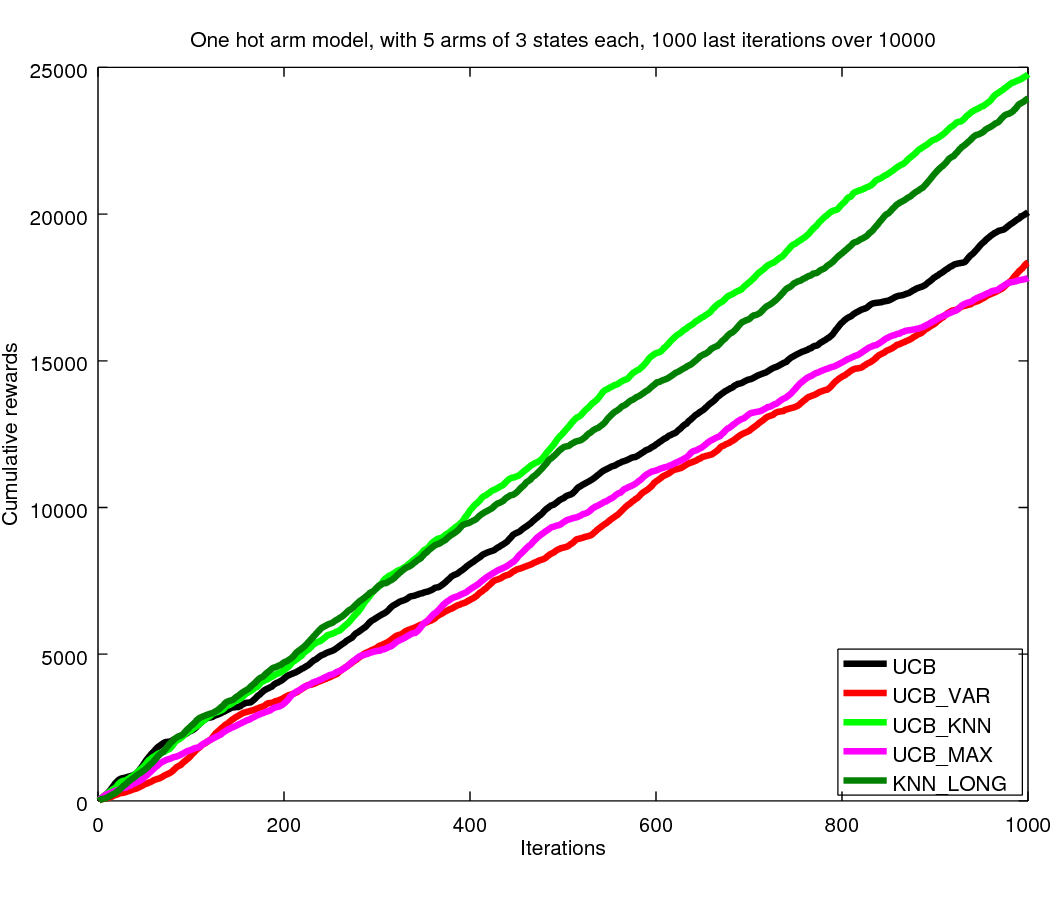
\includegraphics[width=1.0\textwidth]{last_s_1000it.png}

			\centering{\scriptsize{1000 last iterations (5*3, one)}}
		\end{minipage}
		\label{fig:f}
	\end{figure}
\end{frame}

\begin{frame}
	\frametitle{Results (Several hot arms, 5 arms * 3 states)}

	\begin{figure}[h]
		\begin{center}
			%\framebox[4.0in]{$\;$}
			%\fbox{\rule[-.5cm]{0cm}{4cm} \rule[-.5cm]{4cm}{0cm}}
			\vspace{-10pt}
			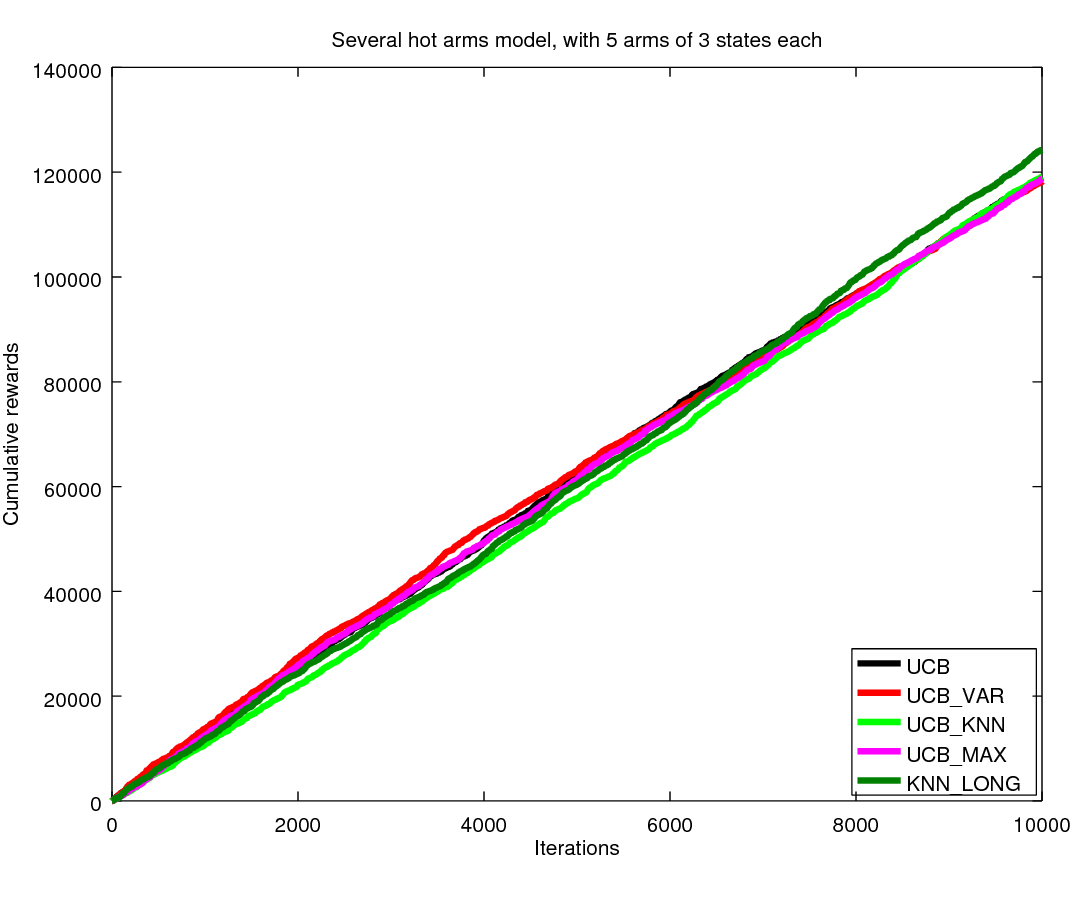
\includegraphics[width=1.05\textheight]{all_ms_10000it.png}

			\vspace{-10pt}
			\centering{\scriptsize{All algorithms for 10000 iterations (5 arms * 3 states, several hot arms)}}
		\end{center}
	\end{figure}
\end{frame}

\begin{frame}
	\frametitle{Results (Several hot arms, 5 arms * 3 states)}

	\begin{figure}[h]
		\begin{minipage}[b]{.49\linewidth}
			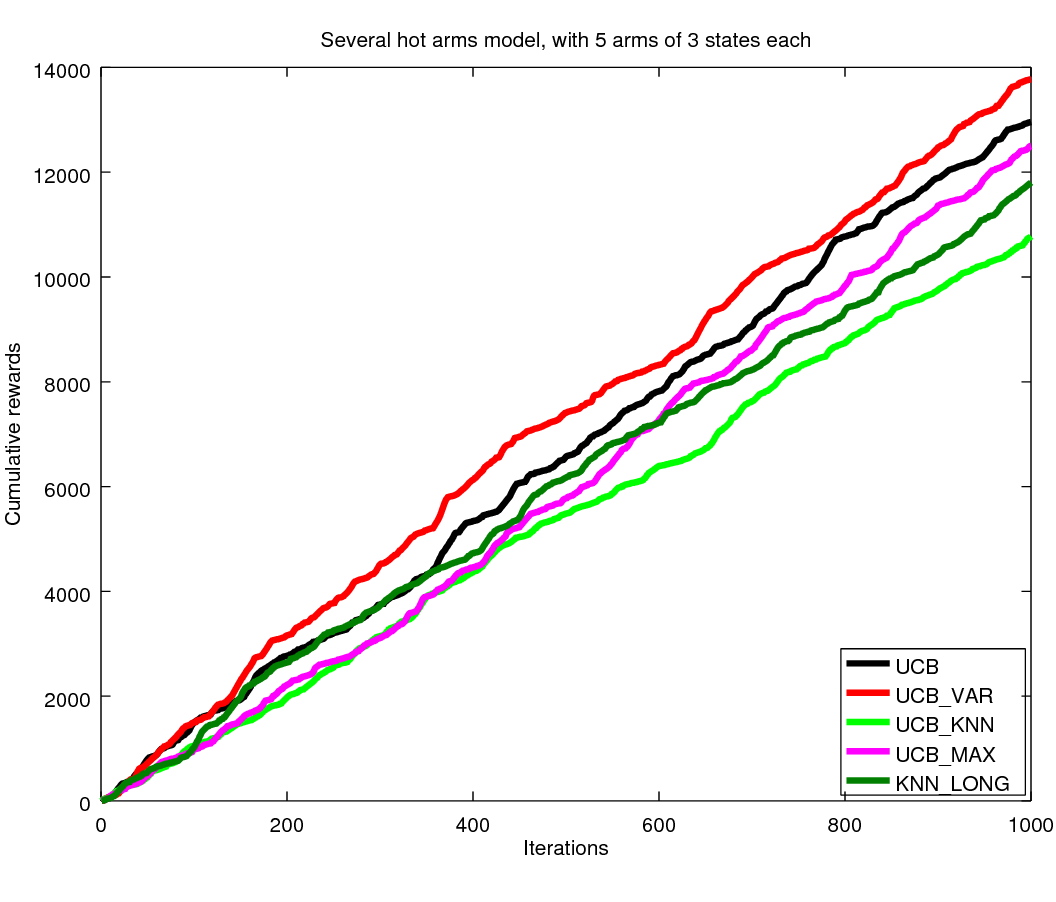
\includegraphics[width=1.0\textwidth]{begin_ms_1000it.png}

			\centering{\scriptsize{1000 first iterations (5*3, several)}}
		\end{minipage}
		\hfill
		\begin{minipage}[b]{0.49\linewidth}
			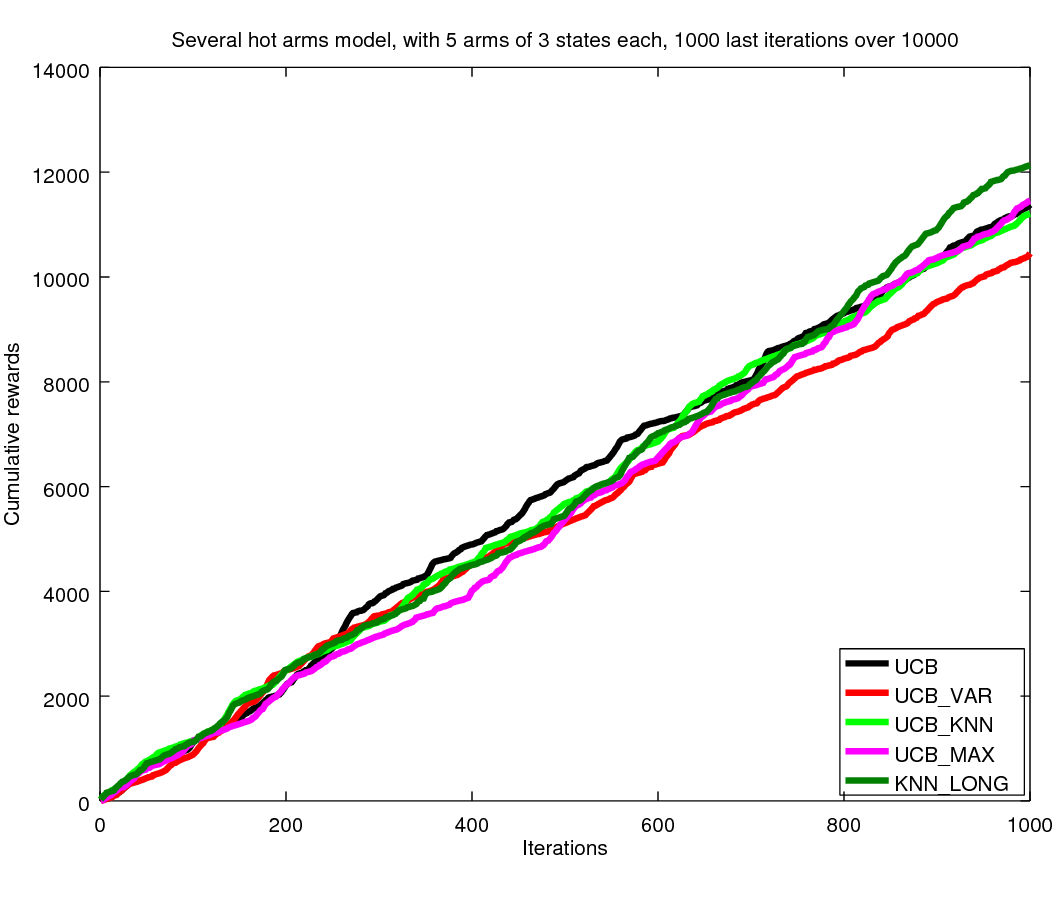
\includegraphics[width=1.0\textwidth]{last_ms_1000it.png}

			\centering{\scriptsize{1000 last iterations (5*3, several)}}
		\end{minipage}
		\label{fig:f}
	\end{figure}

\end{frame}

\begin{frame}
	\frametitle{Conclusion}

	\section{Conclusion}

	\begin{itemize}
		\item UCB misses high rewards as they explore less over time.

		\item UCB\_Var and UCB\_Max : good but don't improve over time.

		\item UCB\_KNN : good at the end but have a long initialization.

		\item KNN\_LONG performs better with several hot arms.
	\newline
	\end{itemize}

$\rightarrow$ Compute greedy algorithm for the next $n$ draws instead of one ?
$\rightarrow$ Try arms that do not follow a Gaussian distribution ?

\end{frame}

\begin{frame}
	\frametitle{references}


	\small{
		\begin{itemize}
		\item [1] Auer, P., Cesa-Bianchi, N., \& Fischer, P. (2002). Finite-time analysis of the multiarmed bandit problem. Machine learning, 47(2-3), 235-256.

		\item [2] Agrawal, S., \& Goyal, N. (2012, June). Analysis of Thompson Sampling for the Multi-armed Bandit Problem. In COLT (pp. 39-1).
		\end{itemize}
	}
\end{frame}

	\begin{frame}
	\frametitle{Thanks}

	Thank you for your attention !

	\end{frame}

\end{document}
